\documentclass[11pt]{article}
\usepackage[margin=1in]{geometry}
\usepackage[T1]{fontenc}\usepackage{lmodern}
\usepackage{amsmath,graphicx,booktabs,enumitem}
\usepackage[authoryear,round]{natbib}
\usepackage{xurl}
\usepackage[dvipsnames]{xcolor}
\usepackage[colorlinks=true,linkcolor=MidnightBlue,citecolor=MidnightBlue,urlcolor=MidnightBlue]{hyperref}
\usepackage{setspace}\setstretch{1.12}
\bibliographystyle{plainnat}
\title{Is 3--1 the Most Dangerous Lead in Hockey?\\[2pt]\large Evidence from 125,000 In-Game Leads and 800 Playoff Series}
\author{Dubya\thanks{Data and code: \texttt{nhl-blown-leads/} in the accompanying repository. All data are from the NHL's public APIs, collected 31 October 2026.}}
\date{31 October 2026}
\begin{document}\maketitle

\begin{abstract}\noindent
Hockey folklore holds that certain leads are cursed: ``2--0 is the worst lead in hockey,'' and, since Cleveland's 2016 comeback in the NBA Finals, ``the 3--1 lead.'' I test these beliefs using every goal from 27,230 NHL games (2005--06 to October 2026), covering 125,106 lead situations, and every best-of-seven NHL playoff series since 1939 (801 series). Inside a game, the particular score does not matter. Once the size of the lead, the time remaining, home ice and team strength are held fixed, a 3--1 lead is exactly as safe as 2--0, 4--2 or 5--3: the odds ratio for 3--1 against 2--0 is 0.96 ($p=0.36$). Whether the lead was reached by the leader scoring or by the trailer cutting a bigger lead makes no difference either, so there is no ``momentum'' effect. The 2--0 myth has a simple explanation. A 2--0 lead is usually reached earlier in the game than a 3--1 lead, so it has more time to be lost: it is tied up 30 per cent of the time against 19 per cent for 3--1, a gap that disappears once time is controlled for. In playoff series, a 3--1 lead is among the safest positions in the sport. It has been blown 32 times in 361 series (8.9 per cent), below both a coin-flip benchmark (12.5 per cent) and a model based on team strength and home ice (11.3 per cent). The weakest ``advantage'' I find is a 2--1 series lead. It is converted only 69 per cent of the time, essentially the same as a 1--0 lead (68 per cent), and it is the only series lead that does not outperform the strength model. Inside games, the weakest is a one-goal lead in a high-scoring game: a team leading 4--3 after two periods loses 30 per cent of the time, against about 24 per cent for other one-goal leads.
\end{abstract}

\section{Introduction}

Few sports are as rich in folk statistics as hockey. Broadcasters warn that a 2--0 lead is ``the most dangerous lead in hockey,'' on the theory that the leading team relaxes while the trailing team needs only one goal to ``get back in it.'' Since the Cleveland Cavaliers came back from 1--3 down against Golden State in the 2016 NBA Finals, ``blew a 3--1 lead'' has become shorthand across sport for a collapse from a commanding position. In hockey the phrase is ambiguous. It can mean a 3--1 score inside a game or a 3--1 lead in a best-of-seven series, so this paper tests both.

The questions are simple. (1) Is any particular score inside a game more dangerous than others with the same lead and the same time left? (2) Does the way a score was reached matter, as ``momentum'' stories claim? (3) How often are series leads blown, and is 3--1 special? (4) Taking everything together, what is the worst ``advantageous'' position in hockey?

The answers are mostly deflationary, which is itself the finding. Inside a game, the chance of blowing a lead depends on two things only: how big the lead is and how much time is left. The scoreline itself carries no information beyond that, and neither does momentum, a result in the spirit of the hot-hand literature \citep{gvt1985,millersanjurjo2018}. The folklore arises from comparing leads that occur at different times. The 3--1 series lead, far from cursed, is one of the most reliable positions in the sport.

\section{Data}

\paragraph{In-game.} For every completed regular-season and playoff game from 2005--06, the first season without ties, to 30 October 2026, I collected the scoring summary from the NHL's gamecenter API \citep{nhlapi}. That gives 27,230 games and every goal with its period, time, team and running score. One game with an inconsistent sequence was dropped. Shootout goals are excluded from the goal sequence, but the shootout winner counts as the winner of the game.

Because scores only increase, each exact score (say 3--1) can occur at most once per game. For every leading score I record:
\begin{itemize}[itemsep=1pt]
\item when it was first reached;
\item whether the leader \emph{extended} to it (2--1 to 3--1) or the trailer \emph{cut} to it (3--0 to 3--1);
\item whether the lead was later \emph{lost}, meaning the game was tied at some point;
\item whether the leading team lost the game, in regulation, overtime or a shootout.
\end{itemize}
There are 125,106 such lead situations. Team strength is each team's regular-season points percentage, and the strength difference between leader and trailer is a control.

\paragraph{Series.} From the NHL's game archive I rebuilt every playoff series from game results. The series identifier is decoded from the game ID. I kept the 801 best-of-seven series, 1939--2026, in which the winner reached four wins with no tied games. The data reproduce the historical record of full comebacks from 0--3 down exactly (1942 Toronto, 1975 New York Islanders, 2010 Philadelphia, 2014 Los Angeles).

Each series lead is compared with two benchmarks. The first treats every game as a coin flip. The second uses a strength model: each game's win probability comes from a logit on the two teams' regular-season points-percentage difference and home ice, estimated on all playoff games, and is then rolled forward through the remaining games of the series with the 2--2--1--1--1 home-ice pattern.

\section{Results inside games}

\paragraph{Raw rates.} Table~\ref{tab:ingame} reports, for each leading score, how often the lead was later lost and how often the leader lost the game. Raw rates seem to support the folklore. A 2--0 lead is tied up 30 per cent of the time and turned into a loss 15 per cent of the time, against 19 and 9 per cent for a 3--1 lead. But the ``Min.\ left'' column shows why. The average 2--0 lead is reached with 38 minutes remaining, the average 3--1 lead with 23. A lead reached earlier has more time to be lost.

\paragraph{Holding time fixed.} Figure~\ref{fig:curves} plots the leader's probability of losing against the time remaining when the score was reached. Within each lead size, the curves for different scores lie on top of one another. In a logit of losing on lead size interacted with a quadratic in time remaining, plus home ice and team strength, the observed loss rate for every common score (each occurring in more than 4,000 games) falls within 3 per cent of its expected rate (Table~\ref{tab:ingame}, last two columns). The larger ratios for rare, lopsided scores such as 5--1 and 5--2 rest on a handful of losses.

The direct tests are scores with the same lead. Among two-goal leads, 3--1 has odds of losing 0.96 times those of 2--0 ($p=0.36$); 4--2 has 1.06 ($p=0.41$); 5--3 has 1.00. Among one-goal leads, 2--1, 3--2 and 4--3 differ from 1--0 by 1--3 per cent in odds, with no difference close to significant. A 3--1 lead is in fact very slightly \emph{safer} than its lead and time predict (observed/expected = 0.97). It is not the most dangerous lead in the game.

\paragraph{No momentum.} A 3--1 lead reached by the trailing team scoring (3--0 to 3--1) is no more fragile than one reached by the leader scoring (2--1 to 3--1): a 9.9 against 9.2 per cent loss rate, and part of that gap reflects time. Pooling 2--1, 3--1, 3--2, 4--1 and 4--2 with controls, the ``cut'' coefficient is 0.003 (s.e.\ 0.027). The goal that narrows a lead carries no information beyond the new score and the clock.

\paragraph{Scoring level.} One pattern survives. Entering the third period, one-goal leads hold equally well at 1--0, 2--1 and 3--2 (leaders lose 24.4--24.5 per cent), but a 4--3 lead is lost 30.0 per cent of the time ($n=586$; Figure~\ref{fig:third}). Across all one-goal leads entering the third, each additional goal already scored raises the leader's chance of losing slightly (logit $+0.025$ per goal, $p=0.054$). That is consistent with high-scoring games having higher remaining scoring rates, because of weak goaltending or open play. The effect is small, and there is no comparable effect for two-goal leads.

\paragraph{A practical lookup.} Because only lead size and time matter, a two-way table summarises in-game risk (Table~\ref{tab:lookup}). A one-goal lead reached with 40--60 minutes left is lost a third of the time. A two-goal lead reached in the last ten minutes is almost never lost (2.3 per cent with 5--10 minutes left, 0.3 per cent inside five minutes). The playoff numbers are close to the regular-season ones (Appendix Table~\ref{tab:playoffs}).

\begin{table}[t]\centering\small
\caption{Every leading score, regular season 2005--06 to October 2026}\label{tab:ingame}
\begin{tabular}{lrrrrrr}\toprule
Score & Games & Min.\ left & Lead lost (\%) & Leader lost (\%) & Expected (\%) & Obs./Exp.\\\midrule
1-0 & 25,379 & 48 & 64.5 & 32.4 & 32.3 & 1.00\\
2-1 & 17,513 & 31 & 54.5 & 27.3 & 27.5 & 0.99\\
3-2 & 10,343 & 19 & 43.7 & 21.8 & 21.6 & 1.01\\
4-3 & 4,261 & 13 & 35.3 & 18.3 & 17.8 & 1.03\\
2-0 & 12,295 & 38 & 30.0 & 15.1 & 15.0 & 1.01\\
3-1 & 10,508 & 23 & 19.1 & 9.3 & 9.6 & 0.97\\
4-2 & 6,215 & 14 & 12.2 & 6.1 & 5.7 & 1.06\\
5-3 & 2,493 & 9 & 7.5 & 3.7 & 3.7 & 1.01\\
3-0 & 5,875 & 29 & 9.6 & 4.6 & 4.6 & 1.00\\
4-1 & 5,621 & 17 & 4.9 & 2.5 & 2.3 & 1.07\\
5-2 & 3,195 & 10 & 2.2 & 0.9 & 1.1 & 0.79\\
4-0 & 2,534 & 24 & 2.0 & 1.0 & 1.0 & 0.99\\
5-1 & 2,249 & 16 & 1.4 & 0.5 & 0.5 & 1.17\\
\bottomrule\end{tabular}
\begin{minipage}{0.95\linewidth}\footnotesize\vspace{4pt}
\emph{Notes:} ``Games'' is the number of games in which the score occurred. ``Min.\ left'' is the mean regulation time remaining when it first occurred. ``Lead lost'' means the game was later tied. ``Leader lost'' means the leading team lost in regulation, overtime or a shootout. ``Expected'' comes from a logit on lead size $\times$ (time remaining, time remaining$^2$), home ice and team-strength difference. Obs./Exp.\ above one means the score is more dangerous than its lead and time imply.
\end{minipage}
\end{table}

\begin{figure}[t]\centering
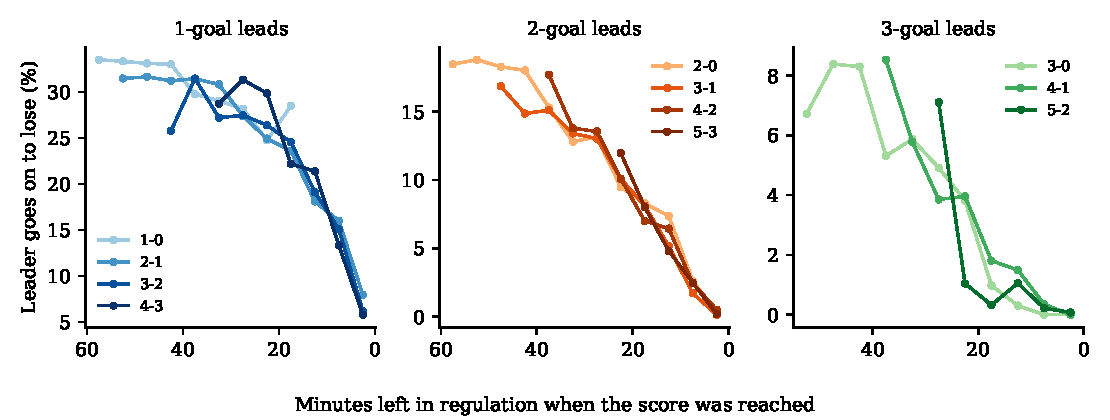
\includegraphics[width=\linewidth]{../analysis/figures/fig_ingame_curves.pdf}
\caption{Probability that the leading team goes on to lose, by the score and the minutes remaining when that score was reached (regular season, 5-minute bins, cells with at least 150 games). Different scores with the same lead fall on the same curve.}\label{fig:curves}
\end{figure}

\begin{figure}[t]\centering
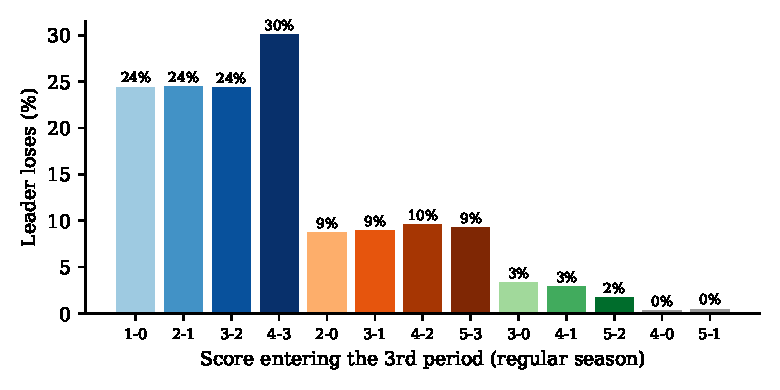
\includegraphics[width=0.78\linewidth]{../analysis/figures/fig_entering_third.pdf}
\caption{Share of games lost by the team leading after two periods, by score (regular season).}\label{fig:third}
\end{figure}

\begin{table}[t]\centering\small
\caption{Chance the leader loses (\%), by lead size and minutes left in regulation when the lead score was reached}\label{tab:lookup}
\begin{tabular}{lrrrrr}\toprule
Minutes left & 40--60 & 20--40 & 10--20 & 5--10 & 0--5\\\midrule
1-goal lead & 32.9 & 28.7 & 21.7 & 14.5 & 6.5\\
2-goal lead & 17.9 & 12.9 & 6.8 & 2.3 & 0.3\\
3-goal lead & 7.7 & 4.8 & 1.2 & 0.2 & 0.0\\
\bottomrule\end{tabular}
\end{table}

\section{Results for playoff series}

Table~\ref{tab:series} and Figure~\ref{fig:series} show every series lead. Three findings stand out.

\paragraph{The 3--1 series lead is safe.} Teams up 3--1 have won 329 of 361 series. The 32 collapses include the four full 0--3 comebacks, which passed through 3--1, and famous recoveries such as the 1987 Islanders against Washington, Minnesota's two comebacks in 2003, Montreal over Toronto in 2021, and Florida over Boston in 2023. The 8.9 per cent blow rate is below the 12.5 per cent a coin flip implies and below the 11.3 per cent the strength model implies. Since 1987 the rate is 10.5 per cent (28 of 267), again below both benchmarks. The 3--1 lead is not cursed. Its collapses are memorable because they are rare.

\paragraph{Leaders are better than they look.} Every series lead except 2--1 is held more often than the strength model predicts. The gap is largest for 3--0 (4 of 218 blown, 1.8 per cent, against an expected 4.8 per cent; $p=0.04$). A team that wins the first three games has revealed that it is stronger than its regular-season record suggested, so the leader's edge is larger than either benchmark assumes.

\paragraph{The weakest advantage: up 2--1.} A 2--1 series lead is converted 69.0 per cent of the time, almost exactly the same as a 1--0 lead (68.2 per cent), and it is the only lead blown \emph{more} often than the strength model predicts (31.0 against 29.8 per cent; since 1987, 32.5 against 30.2 per cent). The excess is not statistically significant. The practical point stands: winning game three after splitting the first two moves a team's series chances about as much as winning game one did, and much less than fans tend to assume. Going up 2--0 is worth far more (86 per cent).

\begin{table}[t]\centering\small
\caption{How often series leads are blown, best-of-seven NHL playoff series}\label{tab:series}
\begin{tabular}{lrrrrrr}\toprule
Lead & Series & Blown & Blown (\%) & Coin-flip (\%) & Model (\%) & $p$\\\midrule
\multicolumn{7}{l}{\emph{All eras (1939--2026)}}\\
Up 1-0 & 801 & 255 & 31.8 & 34.4 & 31.3 & 0.76\\
Up 2-0 & 424 & 58 & 13.7 & 18.8 & 15.7 & 0.29\\
Up 2-1 & 583 & 181 & 31.0 & 31.2 & 29.8 & 0.50\\
Up 3-0 & 218 & 4 & 1.8 & 6.2 & 4.8 & 0.04\\
Up 3-1 & 361 & 32 & 8.9 & 12.5 & 11.3 & 0.16\\
Up 3-2 & 468 & 94 & 20.1 & 25.0 & 23.6 & 0.07\\
\multicolumn{7}{l}{\emph{1987--2026}}\\
Up 1-0 & 570 & 194 & 34.0 & 34.4 & 32.8 & 0.53\\
Up 2-0 & 280 & 38 & 13.6 & 18.8 & 16.6 & 0.20\\
Up 2-1 & 434 & 141 & 32.5 & 31.2 & 30.2 & 0.30\\
Up 3-0 & 136 & 2 & 1.5 & 6.2 & 5.5 & 0.04\\
Up 3-1 & 267 & 28 & 10.5 & 12.5 & 11.6 & 0.63\\
Up 3-2 & 351 & 74 & 21.1 & 25.0 & 23.8 & 0.26\\
\bottomrule\end{tabular}
\begin{minipage}{0.95\linewidth}\footnotesize\vspace{4pt}
\emph{Notes:} ``Series'' counts series that passed through each lead. ``Coin-flip'' is the blow rate if every remaining game were 50/50. ``Model'' uses per-game win probabilities from a logit on the regular-season points-percentage difference and home ice (2--2--1--1--1 format). $p$ is a two-sided binomial test of the observed blow count against the model rate.
\end{minipage}
\end{table}

\begin{figure}[t]\centering
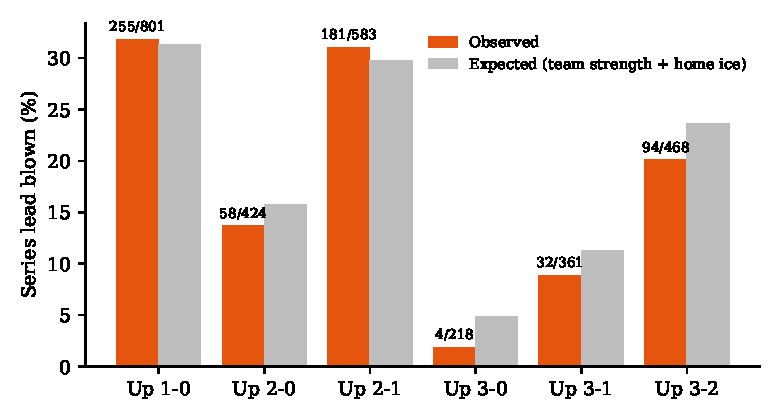
\includegraphics[width=0.78\linewidth]{../analysis/figures/fig_series.pdf}
\caption{Observed against expected blow rates for each series lead, 1939--2026. Labels give blown/total.}\label{fig:series}
\end{figure}

\section{So what is the worst ``advantageous'' position in hockey?}

It depends on what ``worst'' means.

\begin{enumerate}[itemsep=2pt]
\item \textbf{Weakest in absolute terms:} a one-goal lead early in a game. A 1--0 lead reached with more than 40 minutes left is turned into a loss 33 per cent of the time. Among series leads, 1--0 and 2--1 are the weakest: the leader loses roughly 31--32 per cent of them.
\item \textbf{Weakest relative to what it should be worth:} up 2--1 in a series. It is the only series lead that does not beat the strength model, and it is no safer than up 1--0.
\item \textbf{The genuinely shaky in-game lead:} 4--3 after two periods, lost 30 per cent of the time against 24 per cent for any other one-goal lead entering the third. High-scoring games stay volatile.
\item \textbf{Not on the list:} 2--0 or 3--1 in a game, or 3--1 in a series. The 2--0 legend comes from comparing early leads with late ones. The 3--1 legend comes from remembering the 32 collapses and forgetting the 329 conversions.
\end{enumerate}

\section{Limitations}

The in-game panel starts in 2005--06, when ties ended. Before then the ``leader lost'' outcome is not comparable. The strength control is a full-season points percentage, which includes the game itself and ignores injuries, trades and goaltender choice. Empty-net goals are kept, so very late two- and three-goal leads look safer partly because trailing teams pull their goalie. That reflects the real game but should be remembered when reading the lookup table. Series before 1987 mix formats, which is why results are also shown for 1987--2026. Finally, the hot-hand literature warns that conditioning on streaks can bias naive tests \citep{millersanjurjo2018}. The momentum test here compares scores reached by different paths rather than streak lengths, but a formal treatment of path dependence would be a useful extension.

\bibliography{references}

\appendix
\section{Playoff in-game leads}
\begin{table}[h]\centering\small
\caption{Every leading score, playoff games 2006--2026}\label{tab:playoffs}
\begin{tabular}{lrrrr}\toprule
Score & Games & Min.\ left & Lead lost (\%) & Leader lost (\%)\\\midrule
1-0 & 1,851 & 48 & 63.2 & 31.4\\
2-1 & 1,232 & 30 & 52.3 & 25.8\\
3-2 & 705 & 19 & 46.2 & 24.1\\
4-3 & 298 & 13 & 33.9 & 18.8\\
2-0 & 925 & 37 & 30.6 & 15.2\\
3-1 & 712 & 22 & 21.8 & 11.0\\
4-2 & 375 & 12 & 9.9 & 4.3\\
5-3 & 139 & 9 & 3.6 & 2.2\\
3-0 & 439 & 29 & 12.8 & 6.8\\
4-1 & 373 & 15 & 4.0 & 1.9\\
5-2 & 179 & 9 & 1.1 & 0.0\\
4-0 & 199 & 22 & 1.5 & 0.5\\
5-1 & 158 & 13 & 0.6 & 0.0\\
\bottomrule\end{tabular}
\end{table}
\end{document}
